\documentclass[10pt,twocolumn]{article}

\usepackage[margin=0.75in]{geometry}
\usepackage{times}
\usepackage{graphicx}
\usepackage{booktabs}
\usepackage{hyperref}
\usepackage{amsmath}

\title{Plug-and-Play DDIM Sampler Improvement for Official Diffusion Policy Push-T}
\author{Final Project Report}
\date{}

\begin{document}
\maketitle

\begin{abstract}
This project reproduces the official low-dimensional Push-T checkpoint from Diffusion Policy and implements a direct inference-time improvement: replacing the official DDPM ancestral sampler with a DDIM deterministic sampler. The official checkpoint is evaluated with matched Push-T seeds under fixed $(k,h)$ settings, where $k$ is the number of denoising steps and $h$ is the number of executed control steps before replanning. DDIM dramatically improves low/mid-denoising official settings: at $(25,2)$, score improves from 0.155 to 0.900; at $(50,4)$, score improves from 0.653 to 0.929. The claim is carefully bounded: DDIM does not dominate the strongest tested DDPM high-denoising baseline $(100,8)$, which remains at score 0.949.
\end{abstract}

\section{Introduction}

Diffusion Policy~\cite{chi2023diffusion} generates action chunks through iterative denoising and deploys them in a receding-horizon control loop. Its inference behavior depends on the sampler and the deployment parameters: denoising steps $k$ and executed action horizon $h$. The original official Push-T checkpoint uses a DDPM scheduler. A natural improvement idea is to swap the sampler at inference time, without retraining, using DDIM~\cite{song2021ddim}.

This is not claimed as a new diffusion-model algorithm. The contribution is an official-checkpoint validation of a plug-and-play sampler replacement on Push-T.

\section{Related Work and Claim Boundary}

Diffusion Policy introduced action diffusion for visuomotor policy learning~\cite{chi2023diffusion}. DDIM introduced deterministic non-Markovian diffusion sampling~\cite{song2021ddim}. Recent robotics work such as VADF, RA-DP, TIDAL, RTI-DP, and adaptive diffusion replanning already studies adaptive scheduling, replanning, and inference-time compute allocation~\cite{vadf2026,radp2025,tidal2026,rtidp2025,replanning2023}.

Therefore, this project does not claim a new scheduling algorithm. The supported improvement is narrower and directly tested: using DDIM instead of the official DDPM sampler for the public Diffusion Policy Push-T checkpoint.

\section{Official Reproduction}

The official source was acquired through the GitHub codeload archive after repeated clone instability. The checkpoint was downloaded from the Diffusion Policy project server. The preferred 50-seed official DDPM run used official-era \texttt{diffusers==0.11.1} and produced mean score 0.9187. The checkpoint filename reports 0.969, so the remaining gap is reported as an environment-version reproduction gap.

\section{Method}

The official policy object exposes a \texttt{noise\_scheduler}. The improvement replaces the default DDPM scheduler with:

\begin{verbatim}
DDIMScheduler.from_config(
    policy.noise_scheduler.config)
\end{verbatim}

The model weights, normalizer, observation history, action horizon, and environment runner are unchanged. The evaluation script is \texttt{scripts/run\_official\_kh\_grid.py --sampler ddim}. Matched seed analysis is performed by \texttt{scripts/analyze\_official\_sampler\_comparison.py}.

\section{Results}

\begin{table}[h]
\centering
\caption{Matched 20-seed official Push-T comparison.}
\begin{tabular}{lrrrr}
\toprule
$(k,h)$ & DDPM & DDIM & $\Delta$ & Success $\Delta$ \\
\midrule
$(25,2)$ & 0.155 & 0.900 & +0.745 & +0.800 \\
$(50,4)$ & 0.653 & 0.929 & +0.276 & +0.400 \\
$(100,8)$ & 0.949 & 0.900 & -0.048 & -0.050 \\
\bottomrule
\end{tabular}
\end{table}

Paired bootstrap 95\% confidence intervals for score deltas are $[0.593, 0.870]$ for $(25,2)$, $[0.056, 0.488]$ for $(50,4)$, and $[-0.152, 0.007]$ for $(100,8)$.

\begin{figure}[h]
\centering
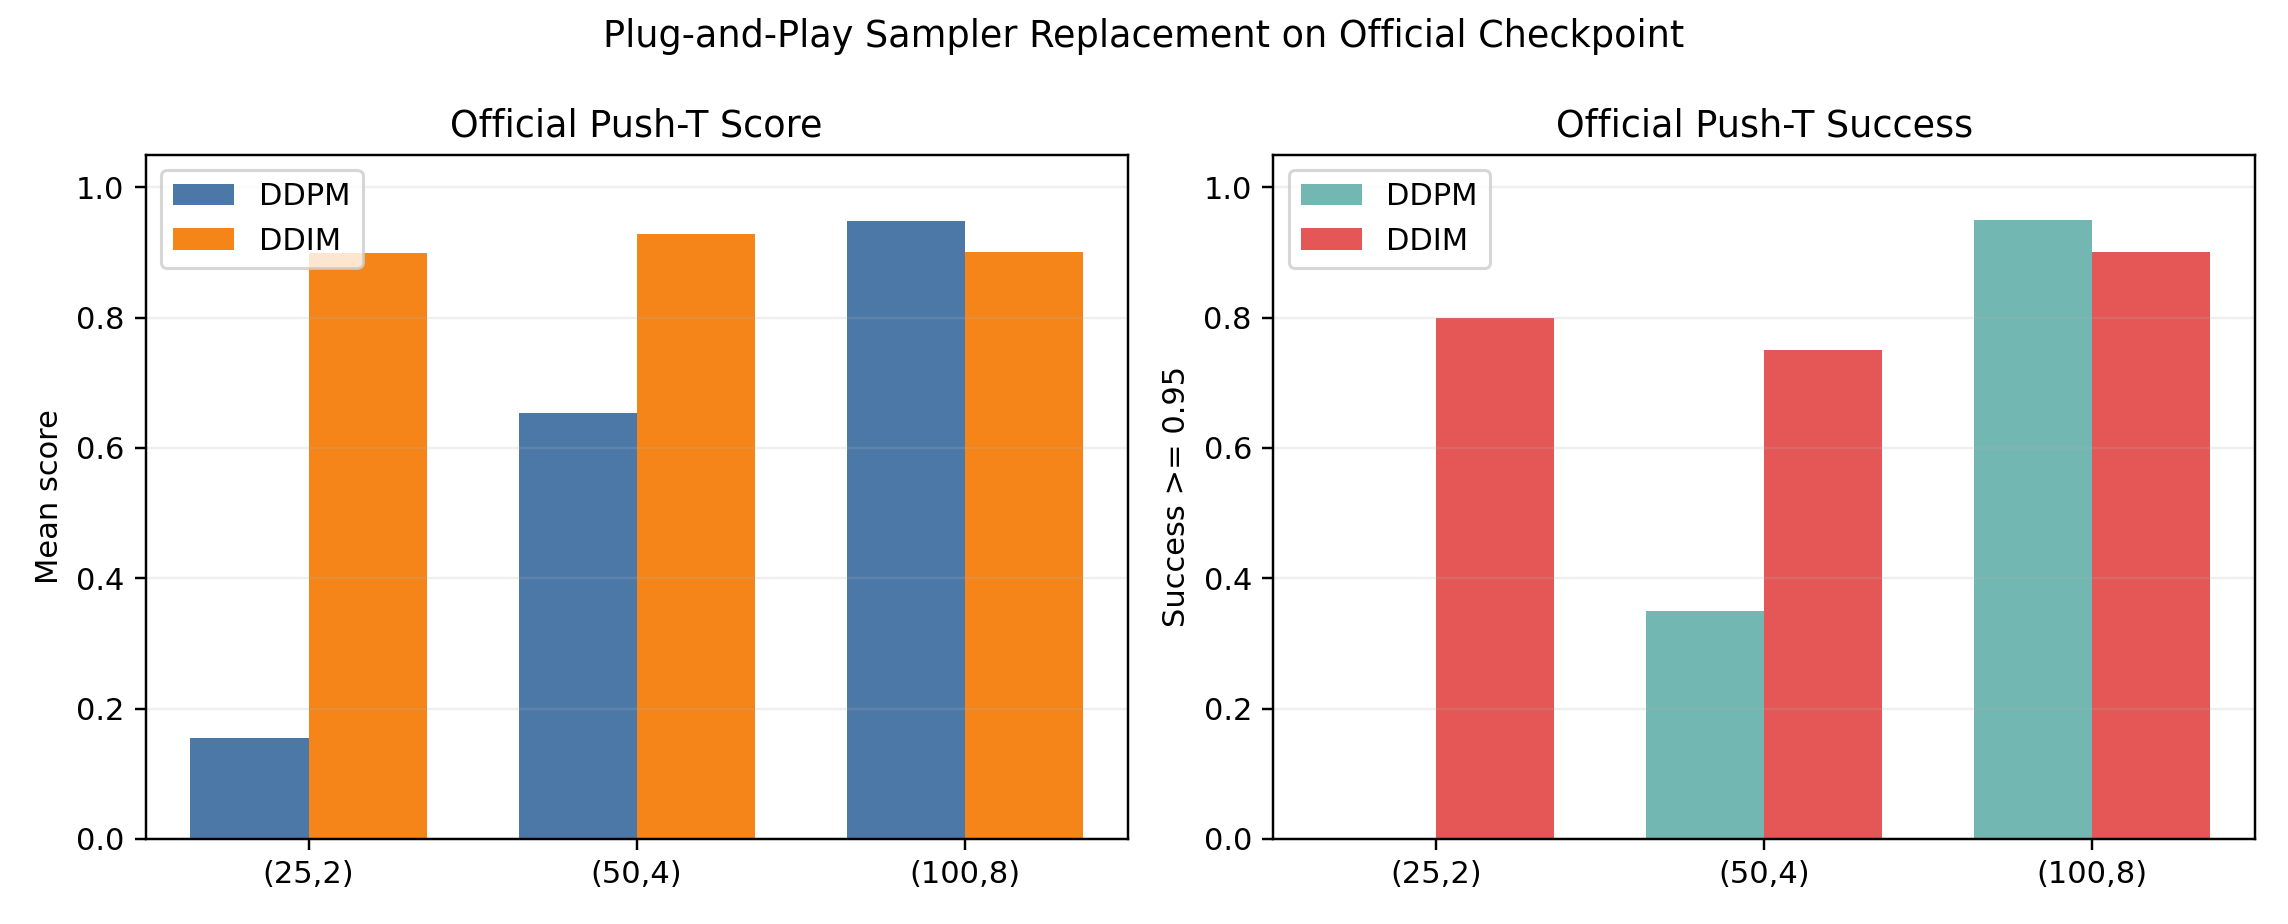
\includegraphics[width=0.95\linewidth]{../figures/official_sampler_comparison.png}
\caption{Plug-and-play DDIM replacement improves low/mid-denoising official checkpoint settings but does not dominate the high-denoising DDPM baseline.}
\end{figure}

\section{Discussion}

DDIM is a strong improvement for low/mid-denoising official checkpoint settings. At $(25,2)$, DDPM nearly fails, while DDIM reaches success 0.800. At $(50,4)$, DDIM nearly matches the high-denoising DDPM baseline in mean score while improving success from 0.350 to 0.750. However, DDIM is not universally better: at $(100,8)$, DDPM remains stronger in this experiment.

\section{Limitations}

The official reproduction uses a compatibility environment rather than the original Python 3.9 / PyTorch 1.12 / Gym 0.21 stack. The DDIM comparison is limited to three high-budget $(k,h)$ settings. Runtime wall-clock speed was not benchmarked separately; NFE is used as the compute proxy. DDIM is an established sampler, so the contribution is application and validation on the reproduced official checkpoint.

\section{Conclusion}

The final project has a defensible improvement result. Starting from an official Diffusion Policy Push-T reproduction, it implements a plug-and-play DDIM sampler replacement and validates it on official checkpoint rollouts. DDIM substantially improves low/mid-denoising settings over the official DDPM sampler on matched seeds, while the original high-denoising DDPM baseline remains strongest.

\bibliographystyle{plain}
\bibliography{corl_references}

\end{document}
